% \section{\rnn Development Context}\label{sec:context}
\section{Online Electron Selection}\label{sec:context}


The optimal performance in the measurement of electrons and photons plays a fundamental role in searches for new particles, in the measurement of Standard Model cross-sections, and in the precise measurement of the properties of fundamental particles such as the Higgs~\cite{HIGG-2012-27,HIGG-2016-33} and W bosons. Here, the electron-based selection is described. As the \rnn{} algorithm was developed for calorimeter signal processing, Section~\ref{sec:atlas_trigger} describes the calorimeter systems in detail with an emphasis on the standard calorimeter variables for electron identification and introduces the ring sums as alternative features envisaging a compact detailed description for shower developments in the calorimeter. The electron triggers are described in Section~\ref{ssec:egamma_trigger}.



\subsection{Calorimetry Based Identification}\label{sec:atlas_trigger}

The calorimeter system covers the pseudorapidity\footnote{ATLAS uses a right-handed coordinate system with its origin at the nominal interaction point (IP) in the centre of the detector and the z-axis along the beam-pipe. The x-axis points from the IP to the centre of the LHC ring, and the y-axis points upward. Cylindrical coordinates (r, $\phi$) are used in the transverse plane, \phi being the azimuthal angle around the beam-pipe. The pseudorapidity is defined in terms of the polar angle $\theta$ as \eta = -$\ln{tan(\theta/2)}$. The angular distance $\Delta R$ is defined as $\Delta R = \sqrt{(\Delta\eta)^{2} + (\Delta\phi)^{2}}$ . Transverse momenta and energies are defined as $pT = p\sin\theta$ and $E_{T}$ = $E\sin\theta$, respectively.} range \(|\eta| < 4.9\)~\cite{PERF-2007-01}. Within the region \(|\eta|< 3.2\),
electromagnetic calorimetry is provided by barrel and endcap high-granularity
lead/Liquid-Argon (LAr) calorimeters, with an additional thin LAr presampler
(\ps) covering \(|\eta| < 1.8\), in order to correct for energy losses in
material upstream of the calorimeters~\cite{LARG-2009-01,larg_tdr}. Hadronic
calorimetry is provided by the steel/scintillating-tile calorimeter
(\tilecal~\cite{TCAL-2017-01,tile_tdr}), constituted of three barrel structures
within \(|\eta| < 1.7\), and two copper/LAr hadronic endcap calorimeters
(\hec)~\cite{cal_tdr}.  The solid angle coverage is completed with forward
copper/LAr and tungsten/LAr calorimeter modules optimised for electromagnetic
(EM) and hadronic (HAD) measurements, respectively. The specified calorimeters
provide full azimuthal ($\phi$) coverage with a total of about 190,000 readout cells. Transition regions between calorimeters are used to locate detector services and induce a sharing of showers between calorimeters that degrades energy measurements in those regions. In particular, the transition from the barrel to the end-cap within
$1.37<|\eta|<1.52$ is complemented by scintillator ($1.0<|\eta|<1.6$) to
estimate signal losses~\cite{cal_tdr}.

The electromagnetic and hadronic calorimeters are segmented~\cite{PERF-2007-01}\footnote{The two
central layers in HCAL end-cap are summed to result in a single measurement.} longitudinally (i.e. in depth) into three sampling layers each. Each sampling layer has its own lateral ($\eta\times\phi$) granularity, for detailed information. Besides granularity, the amount of material in front of the detector in each sampling layer also varies with \abseta, leading to variations in the expected lateral and longitudinal profiles. Additionally, the expected
profile is also dependent on the physics object total energy. In the EM calorimeter, most of the EM shower energy is collected in the second layer, while the third layer provides measurements
of energy deposited in the shower tails. Although, it is important to mention that the first EM layer (EM1) plays an important role in the discrimination of electrons against $\pi^0$. 

The hadronic calorimeters, which surround the EM detectors,
provide additional discrimination power through further energy measurements of
possible EM shower tails, as well as rejection of events with activity of
hadronic origin with three sampling layers. It is worth noting that QCD jets also have a sizeable fraction of their energy deposited in the EM calorimeter from $\pi^{0}\rightarrow\gamma\gamma$
and other prompt hadronic decays to photons and also bremsstrahlung $\gamma$ radiated by quarks.
Although the calorimeters are designed 
to have uniform response for full detector acceptance, there are residual fluctuations 
dependent on the shower development position~\cite{Wigmans2017}.



\subsubsection{Physics-Inspired Calorimetric Electron Identification}\label{ssec:std_variables}

The specificities of the real electron and background interaction processes with
detector instrumentation can be used to construct meaningful and discriminative physics variables. Except for the hardware-based calorimeter trigger
and the \rnn (Section~\ref{sec:neuralringer}), electron
identification~\cite{atlas_electron_id_offline} relies on the variables
described in Table~\ref{tab:IDcuts}. 
%A schematic illustration of the ATLAS components employed on these variables can be seen in Figure~\ref{fig:schematic_id_inputs}. 
The cut-based algorithm in electron
triggers applies thresholds on the three most discriminating variables discussed in Table~\ref{tab:IDcuts}, which describe important features of the shape of the electromagnetic showers: \reta{}, \eratio{}, \rhadone{}.





\begin{table}[]
\caption{Type and description of the quantities used in electron
  identification.  The columns labelled ``Rejects'' indicate whether a quantity
  is used to discriminate prompt electrons from light-flavour (LF) jets, photon
  conversions ($\gamma$), or non-prompt electrons from the semileptonic decay of
  hadrons containing heavy-flavour (HF) quarks ($b$- or $c$-quarks).  In the
  column labelled ``Usage,'' an ``LH'' indicates that the probability density
  estimation (pdf) of this quantity
  is used in forming $\mathcal{L}_{s}$ and $\mathcal{L}_{b}$ (defined in
  Eq.~(\ref{eq:likelihoods})) and a ``C'' indicates that this quantity is used
  directly as a selection criterion.  In the description of the quantities
  formed using the second layer of the calorimeter, 3$\times$3, 3$\times$5,
  3$\times$7, and 7$\times$7 refer to areas of $\Delta\eta \times \Delta\phi$
  space in units of $0.025 \times 0.025$. Adapted from~\cite{aaboud2019electron}
}%
\label{tab:IDcuts}

\scriptsize
%\renewcommand{\arraystretch}{1.}
\begin{center}
\resizebox{\textwidth}{!}{%
\begin{tabular}{|c|l|c|ccc|c|}
\hline
Type            & \multicolumn{1}{c|}{Description}                                                                        & Name                & \multicolumn{3}{c|}{Rejects}                                 & Usage \\
                &                                                                                                         &                     & \multicolumn{1}{c|}{LF} & \multicolumn{1}{c|}{$\gamma$} & HF &       \\ \hline
Hadronic        & Ratio of \et in the first layer of the hadronic calorimeter                                             & \rhadone            & \multicolumn{1}{c|}{x}  & \multicolumn{1}{c|}{}         & x  & LH    \\
leakage         & to \et of the EM cluster                                                                                &                     & \multicolumn{1}{c|}{}   & \multicolumn{1}{c|}{}         &    &       \\
energy          & (used over the range $|\eta| < 0.8$ or $|\eta| > 1.37$)                                                 &                     & \multicolumn{1}{c|}{}   & \multicolumn{1}{c|}{}         &    &       \\ \cline{2-7} 
                & Ratio of \et in the hadronic calorimeter                                                                &                     & \multicolumn{1}{c|}{}   & \multicolumn{1}{c|}{}         &    &       \\
                & to \et of the EM cluster                                                                                & \rhad               & \multicolumn{1}{c|}{x}  & \multicolumn{1}{c|}{}         & x  & LH    \\
                & (used over the range $0.8 <|\eta| < 1.37$)                                                              &                     & \multicolumn{1}{c|}{}   & \multicolumn{1}{c|}{}         &    &       \\ \hline
Energy in       & Ratio of the energy in the third layer to the total energy in the                                       &                     & \multicolumn{1}{c|}{}   & \multicolumn{1}{c|}{}         &    &       \\
Third layer of  & EM calorimeter. This variable is only used for                                                          &                     & \multicolumn{1}{c|}{}   & \multicolumn{1}{c|}{}         &    &       \\
EM calorimeter  & $\et < \SI{80}{\GeV}$, due to inefficiencies at high \et, and is                                        & \fIII               & \multicolumn{1}{c|}{x}  & \multicolumn{1}{c|}{}         &    & LH    \\
                & also removed from the LH for $|\eta| > 2.37$, where it is                                               &                     & \multicolumn{1}{c|}{}   & \multicolumn{1}{c|}{}         &    &       \\
                & poorly modelled by the simulation.                                                                      &                     & \multicolumn{1}{c|}{}   & \multicolumn{1}{c|}{}         &    &       \\ \hline
Energy in       & Lateral shower width, $\sqrt{(\Sigma E_i \eta_i^2)/(\Sigma E_i) -((\Sigma E_i\eta_i)/(\Sigma E_i))^2}$, &                     & \multicolumn{1}{c|}{}   & \multicolumn{1}{c|}{}         &    &       \\
second layer of & where $E_i$ is the energy and $\eta_i$ is the pseudorapidity                                            & \weta               & \multicolumn{1}{c|}{x}  & \multicolumn{1}{c|}{x}        &    & LH    \\
EM calorimeter  & of cell $i$ and the sum is calculated within a window of 3$\times$5 cells                               &                     & \multicolumn{1}{c|}{}   & \multicolumn{1}{c|}{}         &    &       \\ \cline{2-7} 
                & Ratio of the energy in 3$\times$3 cells over the energy in 3$\times$7 cells                             & \rphi               & \multicolumn{1}{c|}{x}  & \multicolumn{1}{c|}{x}        & x  & LH    \\
                & centred at the electron cluster position                                                                &                     & \multicolumn{1}{c|}{}   & \multicolumn{1}{c|}{}         &    &       \\ \cline{2-7} 
                & Ratio of the energy in 3$\times$7 cells over the energy in 7$\times$7 cells                             & \reta               & \multicolumn{1}{c|}{x}  & \multicolumn{1}{c|}{x}        & x  & LH    \\
                & centred at the electron cluster position                                                                &                     & \multicolumn{1}{c|}{}   & \multicolumn{1}{c|}{}         &    &       \\ \hline
Energy in       & Shower width, $\sqrt{(\Sigma E_i (i-i_\mathrm{max})^2)/(\Sigma E_i)}$, where $i$ runs over              &                     & \multicolumn{1}{c|}{}   & \multicolumn{1}{c|}{}         &    &       \\
first layer of  & all strips in a window of $\Delta\eta \times \Delta\phi \approx 0.0625 \times 0.2$,                     & \wstot              & \multicolumn{1}{c|}{x}  & \multicolumn{1}{c|}{x}        & x  & C     \\
EM calorimeter  & corresponding typically to 20 strips in $\eta$, and $i_\mathrm{max}$ is the                             &                     & \multicolumn{1}{c|}{}   & \multicolumn{1}{c|}{}         &    &       \\
                & index of the highest-energy strip, used for \et\ $>$ 150~\gev\ only                                     &                     & \multicolumn{1}{c|}{}   & \multicolumn{1}{c|}{}         &    &       \\ \cline{2-7} 
                & Ratio of the energy difference between the maximum                                                      &                     & \multicolumn{1}{c|}{}   & \multicolumn{1}{c|}{}         &    &       \\
                & energy deposit and the energy deposit in a secondary                                                    & \deltaEmax          & \multicolumn{1}{c|}{x}  & \multicolumn{1}{c|}{x}        &    & LH    \\
                & maximum in the cluster to the sum of these energies                                                     &                     & \multicolumn{1}{c|}{}   & \multicolumn{1}{c|}{}         &    &       \\ \cline{2-7} 
                & Ratio of the energy in the first layer to the total energy                                              & \fI                 & \multicolumn{1}{c|}{x}  & \multicolumn{1}{c|}{}         &    & LH    \\
                & in the EM calorimeter                                                                                   &                     & \multicolumn{1}{c|}{}   & \multicolumn{1}{c|}{}         &    &       \\ \hline
Track           & Number of hits in the innermost pixel layer                                                             & $n_\mathrm{Blayer}$ & \multicolumn{1}{c|}{}   & \multicolumn{1}{c|}{x}        &    & C     \\ \cline{2-7} 
parameters      & Number of hits in the pixel detector                                                                    & $n_\mathrm{Pixel}$  & \multicolumn{1}{c|}{}   & \multicolumn{1}{c|}{x}        &    & C     \\ \cline{2-7} 
                & Total number of hits in the pixel and SCT detectors                                                     & $n_{\mathrm{Si}}$   & \multicolumn{1}{c|}{}   & \multicolumn{1}{c|}{x}        &    & C     \\ \cline{2-7} 
                & Transverse impact parameter relative to the beam-line                                                   & \trackdO            & \multicolumn{1}{c|}{}   & \multicolumn{1}{c|}{x}        & x  & LH    \\ \cline{2-7} 
                & Significance of transverse impact parameter                                                             & |\dOSignificance|   & \multicolumn{1}{c|}{}   & \multicolumn{1}{c|}{x}        & x  & LH    \\
                & defined as the ratio of \trackdO to its uncertainty                                                     &                     & \multicolumn{1}{c|}{}   & \multicolumn{1}{c|}{}         &    &       \\ \cline{2-7} 
                & Momentum lost by the track between the perigee and the last                                             & \deltapoverp        & \multicolumn{1}{c|}{x}  & \multicolumn{1}{c|}{}         &    & LH    \\
                & measurement point divided by the  momentum at perigee                                                   &                     & \multicolumn{1}{c|}{}   & \multicolumn{1}{c|}{}         &    &       \\ \hline
TRT             & Likelihood probability based on transition radiation in the TRT                                         & \TRTPID             & \multicolumn{1}{c|}{x}  & \multicolumn{1}{c|}{}         &    & LH    \\ \hline
Track--cluster  & $\Delta\eta$ between the cluster position in the first layer                                            & \deltaeta           & \multicolumn{1}{c|}{x}  & \multicolumn{1}{c|}{x}        &    & LH    \\
matching        & and the extrapolated track                                                                              &                     & \multicolumn{1}{c|}{}   & \multicolumn{1}{c|}{}         &    &       \\ \cline{2-7} 
                & $\Delta\phi$ between the cluster position in the second layer                                           &                     & \multicolumn{1}{c|}{}   & \multicolumn{1}{c|}{}         &    &       \\
                & of the EM calorimeter and the momentum-rescaled                                                         & \deltaphires        & \multicolumn{1}{c|}{x}  & \multicolumn{1}{c|}{x}        &    & LH    \\
                & track, extrapolated from the perigee, times the charge $q$                                              &                     & \multicolumn{1}{c|}{}   & \multicolumn{1}{c|}{}         &    &       \\ \cline{2-7} 
                & Ratio of the cluster energy to the track momentum, used for                                             & $E/p$               & \multicolumn{1}{c|}{x}  & \multicolumn{1}{c|}{x}        &    & C     \\
                & \et $>$ 150~\gev\ only                                                                                  &                     & \multicolumn{1}{c|}{}   & \multicolumn{1}{c|}{}         &    &       \\ \hline
\end{tabular}
}

\end{center}

\end{table}





  
The standard electron identification variables are based on an in-depth
understanding of the signatures left by signal and background.  As a result, information in specific regions of the experiment
are fused together using a set of a few variables (i.e. 3 variables for describing the shower shape in the second EM layer). The objective is to reduce the dimensionality of the problem and to compose a highly discriminant input space to apply a set of rectangular cuts, which provides a simple yet powerful selection mechanism. The use of variables providing similar information is discouraged, as they usually do not aggregate with
discriminating power and make analysis more
complex~\cite{aaboud2019electron}.

In the end of the LHC Run~1~\cite{PERF-2016-01}, the strategy for offline electron identification was improved by the adoption of a multivariate approach, which computes a likelihood discriminant. Here, an approximation is made by assuming a statistical independence between variables ~\cite{kendalls_vol2b}. This likelihood approach was also brought to the final HLT selection in Run 2 (Section~\ref{ssec:egamma_trigger}) to improve overall efficiency. 

%In a broader sense, other ATLAS physics objects like taus and jets, for
%which discrimination relies on less prominent instrumentation and carried out on
%similar signal--background interactions, have successfully applied other
%multivariate methods like boosted decision-trees and neural-networks for
%modelling a more suitable and complex decision process.

\newpage

\subsubsection{\rnn{} Based Electron Identification}%\label{ssec:rings_concept}

At each calorimeter sampling layer, the energy deposition of an incoming particle is extracted by building concentric rings of cells (\figurename~\ref{fig:calo_rings}), or simply ``rings''. All rings in the \ecal sampling layers are
centered around their most energetic cell, a reasonable
approximation of the energy barycenter of the shower for online
operation. Focusing on EM objects, rings are built using as axis center the position of the most energetic cell cell in the second electromagnetic layer, collecting the largest fraction of the total absorbed electron energy.


\begin{figure}[h!t]
	\centering
	\begin{center}
		\begin{subfigure}[c]{.95\textwidth}
			\centering
			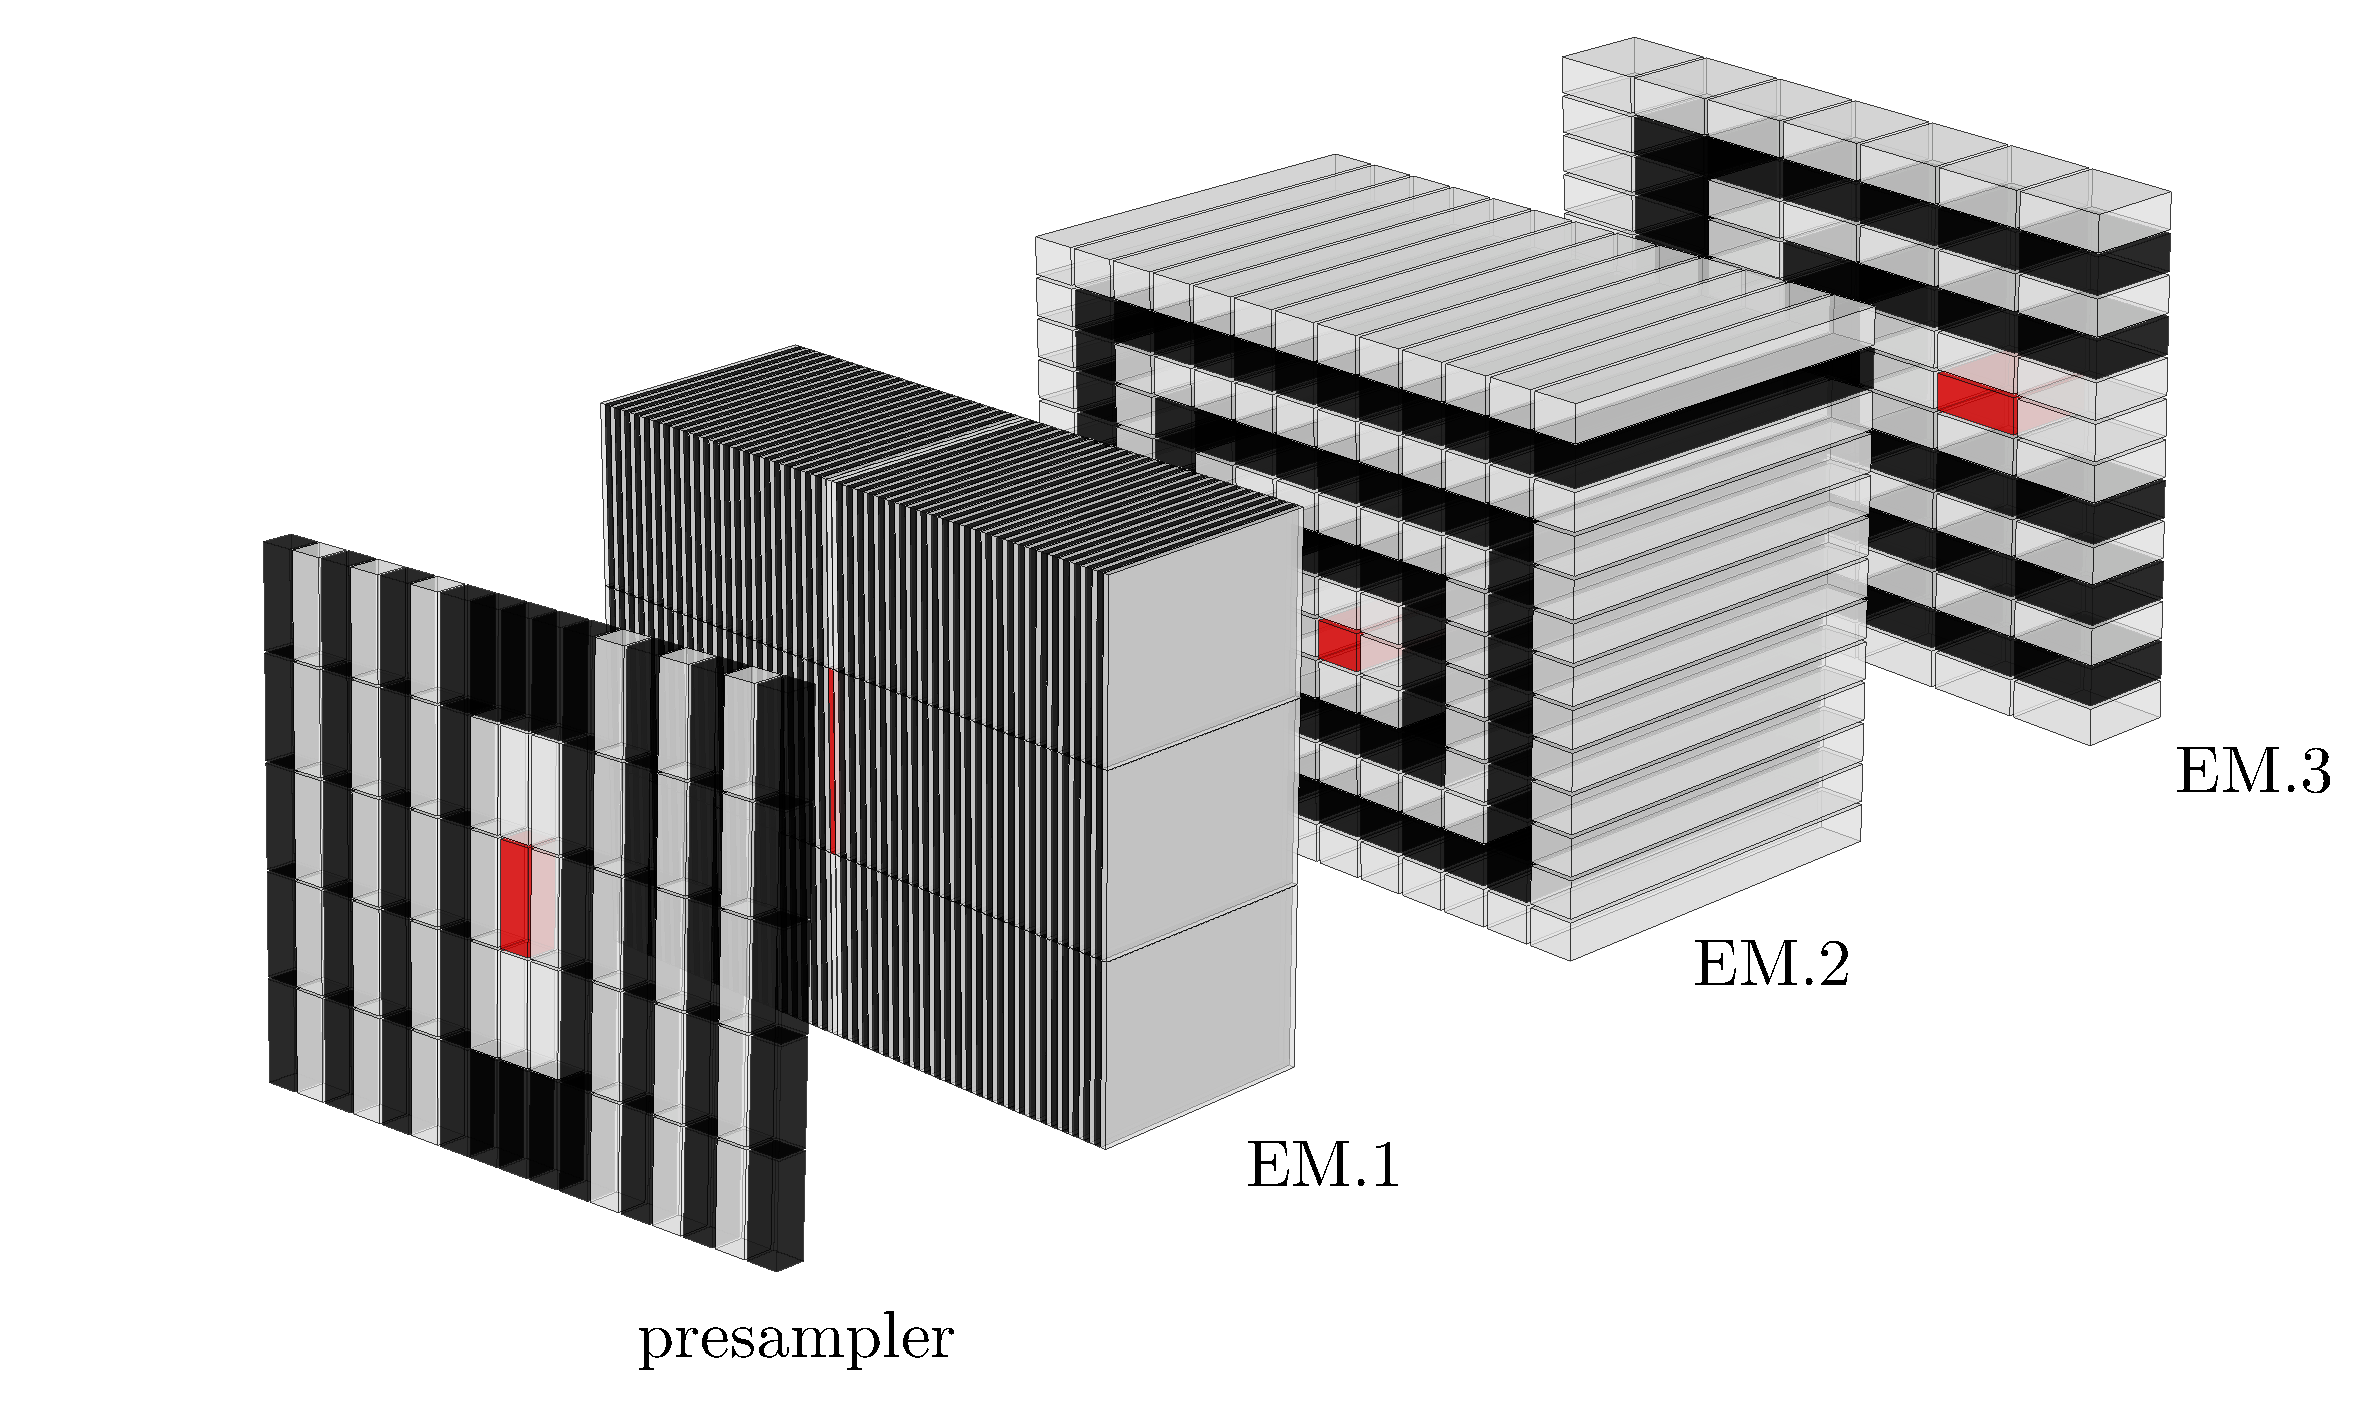
\includegraphics[width=\textwidth]{sections/02_context/figures/ATLAS_EM_Layers_v5.pdf}
			\caption{Eletromagnetic calorimeter cells within the ringer reconstruction window.}
		\end{subfigure} \\
		\begin{subfigure}[c]{.95\textwidth}
			\centering
			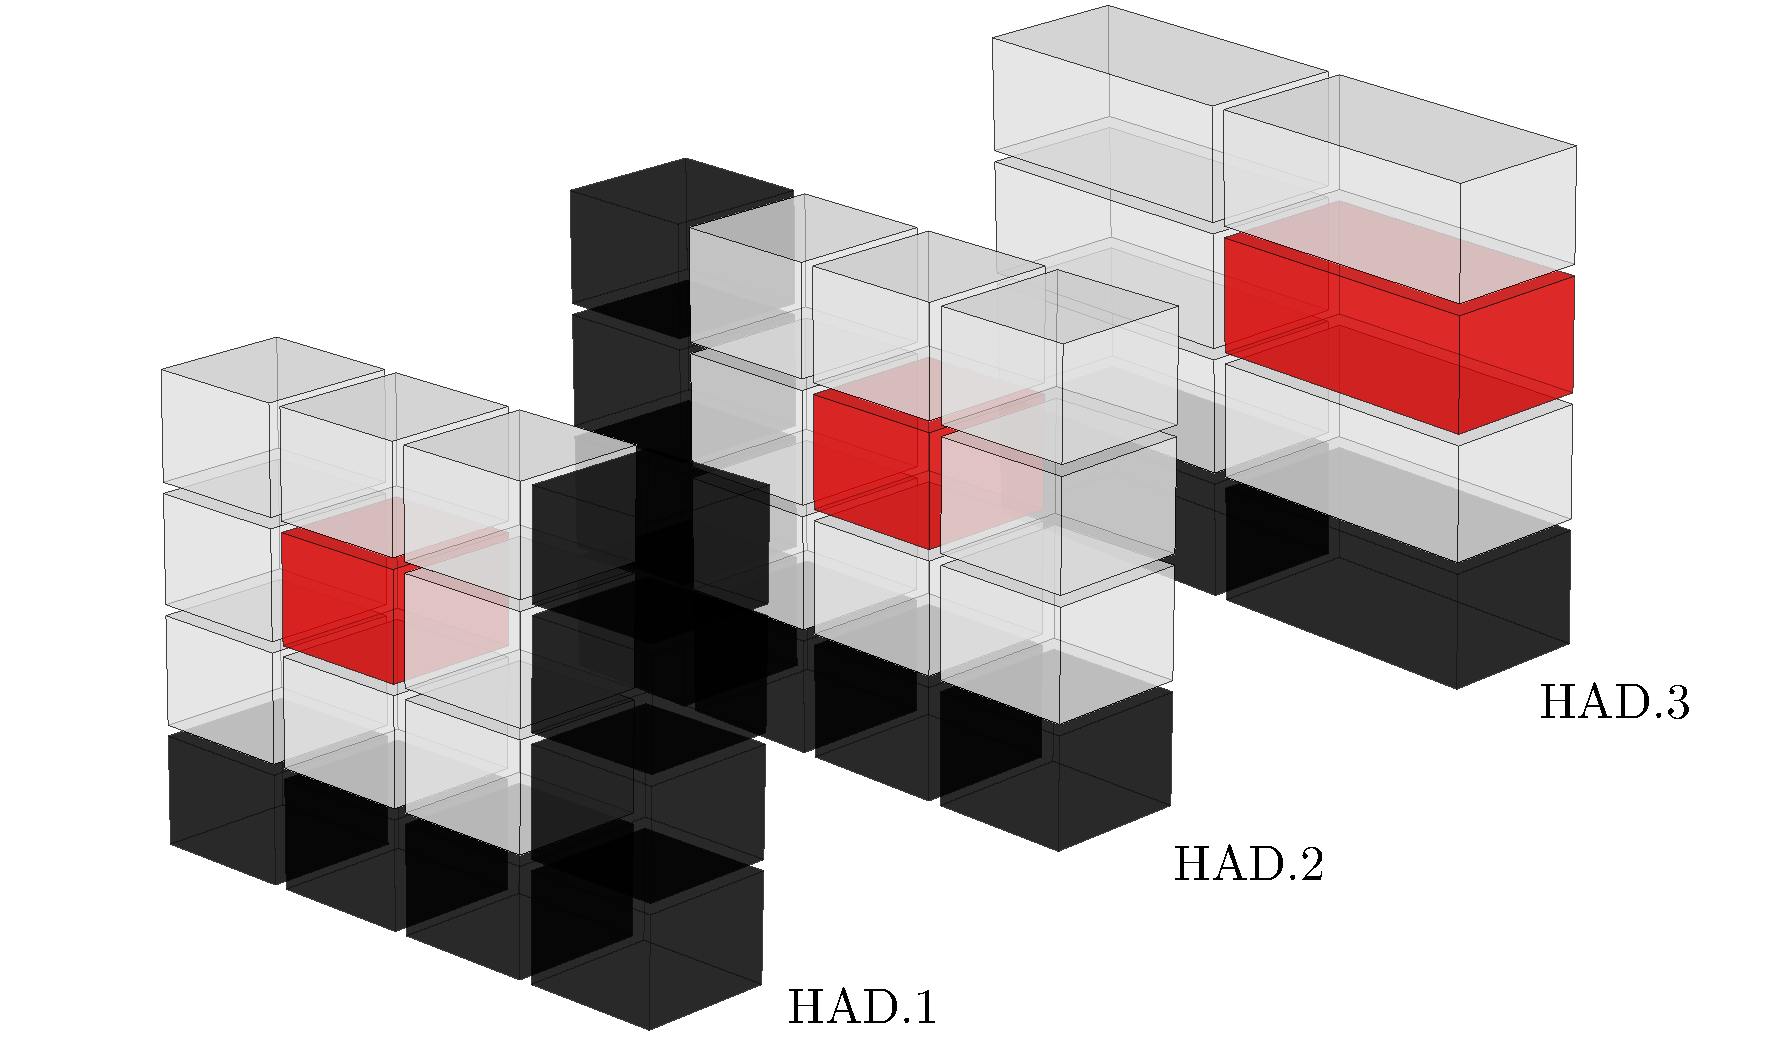
\includegraphics[width=\textwidth]{sections/02_context/figures/ATLAS_HAD_Layers_v5.pdf}
			\caption{Hadronic calorimeter cells within the ringer reconstruction window.}
		\end{subfigure}
	\end{center}
	\caption{\label{fig:calo_rings}
		Sketch to illustrate the ring-shaped energy description. See
		Section~\ref{top:algorithm} for more details. 
		The most energetic cell is in red, while the consecutive neighbouring rings are represented by alternating gray and black cells.
	}
\end{figure}


The ring building process covers the whole $0.4\times0.4$ (\etaphi axis) RoI
seeded by \licalo, resulting in 100 rings in total across all calorimeter layers.
Thereby, a dimensionality reduction is provided by compacting the
typical input space dimensionality of approximately 1000--1200 cells per ROI into
the above-mentioned 100 rings through the usage of EM shower physics knowledge: the rings can keep a complete description of the symmetric lateral and
longitudinal information. However, the algorithm only approximates this concept
in order to meet the online operation requirements and avoid further
manipulation of the instrumented information. The full description and
discussion on the current algorithm are addressed in
Section~\ref{top:algorithm}.



Conceptually, the ring structure aims at exploiting the concentric nature of energy depositions in the calorimeter and the corresponding symmetry in the development of the shower.  Adding the calorimeter cells belonging to a given ring and, thus producing the ring sums, makes it possible to improve the signal-to-noise ratio from individual cells, especially in the tail of the energy distributions along the calorimeter layers.  Moreover, a nonlinear discriminant may profit from the statistical fluctuations in shower development, which are captured by means of the rings' profile, and provide efficient electron selection even in high pileup conditions.

Nonetheless, some observations concerning the description of a shower through rings are worth making. First, the standard shower shape variables, or simply shower shapes, cannot be obtained through operations starting from the rings.  Thus, the rings represent an alternative for shower development description and not a possible replacement for the shower shapes.  Therefore, a strategy considering both rings and shower shapes might explore a complementary discriminating information in the future.



Second, one should also notice
that the rings do not use the same sensors more than once for each variable.
This is not strictly true for the shower shapes, although it is fairly unusual.
In contrast, pattern recognition through modern machine learning
algorithms~\cite{Engelbrecht2007,Goodfellow2016}, such as convolution
neural-networks~\cite{Gu2018}, build variables processing several times
the same sensors. Additionally, as providing dimension reduction and keeping the physics interpretation of the shower development, the shower shapes are also suited to bringing insights through uni-variate analysis carried out on each
single dimension composing the input space.
Thus, an alternative ring-based trigger strategy was developed and the shower shapes were used to evaluate how the physics properties of the showers were captured by the neural networks trained on calorimeter information formatted into ring sums. 









\subsection{Electron Triggers}\label{ssec:egamma_trigger}


Electron triggers~\cite{aad2020performance} begin with
the search for an EM energy deposit in the calorimeter with a \licalo{} sliding
window algorithm ~\cite{Franchino:2730851} using coarse granularity calorimeter information, in order to
fulfill the targeted latency requirements in $2.5\mu s$. This selects a RoI of $0.4\times 0.4$
in the $\eta\times\phi$ plane and applies a minimal transverse energy and object
multiplicity requirements, which depend on the trigger
specifications~\cite{TRIG-2016-01}.
 
The \hlt{} selection starts with the fast calorimeter reconstruction
step (\fastcalo), which has two implementations
(Figure~\ref{fig:ringer_chains}): the original cut-based algorithm; and one based on the Ringer algorithm. 
This processing step is followed by the fast track reconstruction
(\fastelectron), which applies restrictions on variables that indicate the quality of proximity matching between the electron candidate positions reconstructed from the track and the calorimeter. Due to its high-demanding computational algorithms, early removal of fake candidates can be used to reduce the relatively high CPU resources needed for this selection stage.


\begin{figure}[h!tb]
  \begin{center}
  %\hspace{0.01\textwidth}
  \begin{subfigure}[c]{.48\textwidth}
  \centering
  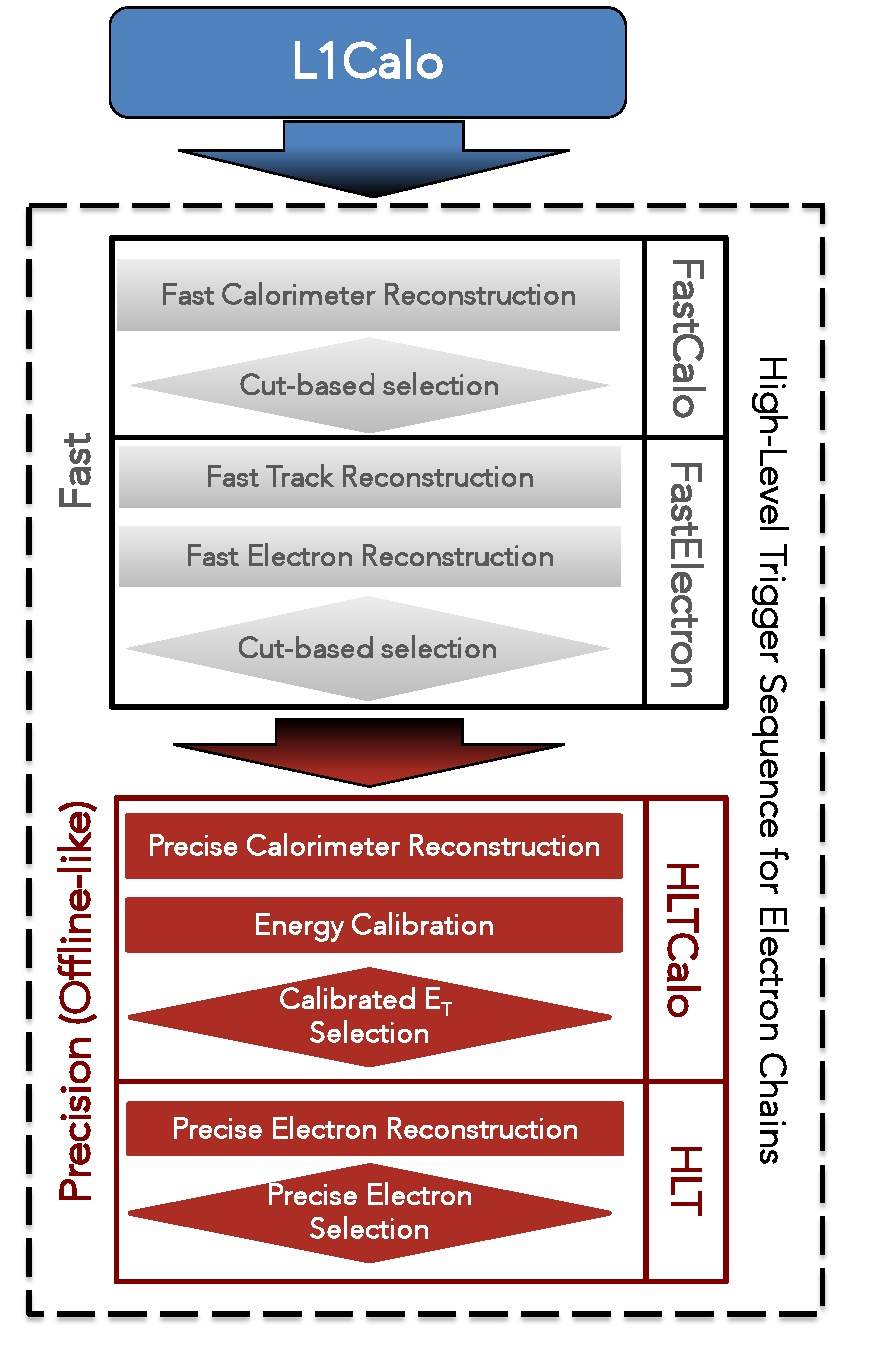
\includegraphics[width=\textwidth]{sections/02_context/figures/ElectronChain_Run2_cutbased.pdf}
  \caption{noringer chain (2017).}
  %\label{fig:cutbased_chain}
  \end{subfigure}
  \hfill
  \begin{subfigure}[c]{.48\textwidth}
  \centering
  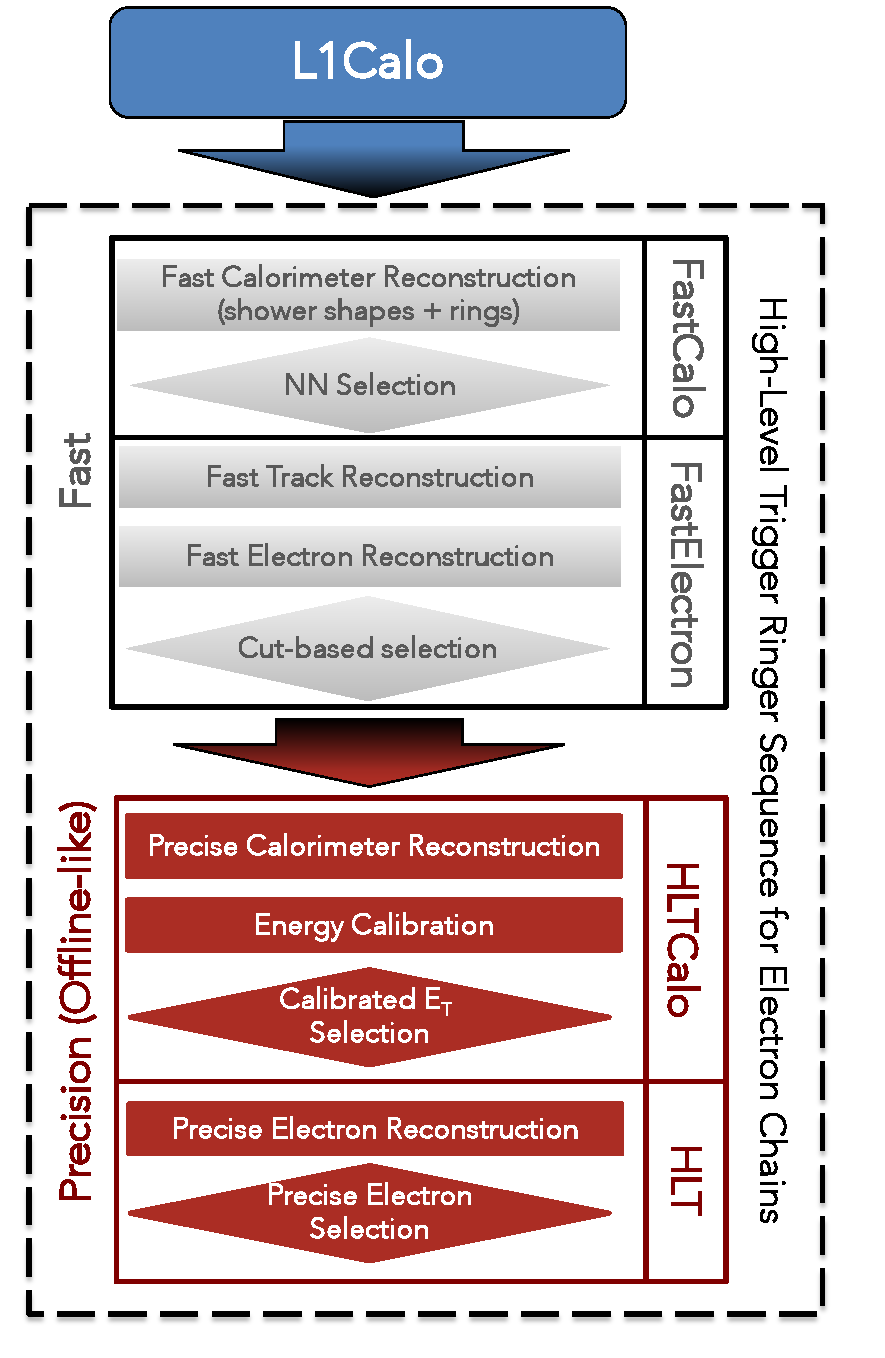
\includegraphics[width=\textwidth]{sections/02_context/figures/ElectronChain_Run2_ringer.pdf}
  \caption{ringer chain (2017).}
  %\label{fig:ringer_chain}
  \end{subfigure}
  %\hfill
  \caption{Comparison of the processing flow diagrams for the electron triggers. (a)
  contains the logic employed in the triggers based on the cut-based strategy
  (noringer) in the \fastcalo step. (b) contains the primary electron
  chains (ringer chains) since 2017, with the \rnn{} algorithm.}%
  \label{fig:ringer_chains}
  \end{center}
\end{figure}

% TODO Remove column (c) or use the note table
  
  

% http://acode-browser1.usatlas.bnl.gov/lxr/source/aa/Trigger/TrigHypothesis/TrigEgammaHypo/python/TrigL2CaloHypoCutDefs.py

A precise electron candidate energy is later computed (\hltcalo). The final HLT selection makes use of a likelihood
approach~\cite{ATL-COM-PHYS-2017-1012,ATLAS-PERF-2017-01-002}, based on the estimation of marginal probability density function (pdf) for the discriminating variables ($\vec{x}$) given in Table~\ref{tab:IDcuts}. The discriminant value is computed by:


%, which is built using adaptive Gaussian Kernel Density Estimation (KDE)~\cite{Silverman2018,TMVA}. The
%resulting kernels, obtained (since 2017) from runs of the previous year, and
%earlier from simulation data, are approximated by histograms with thin
%granularity (generally employing 500 bins) and then interpolated to give the
%signal and background probability values computed for the $i$th variable ($P_{s(b),i}(x_i)$). 


\begin{equation}
  d_{\mathcal{L}} = \frac{\mathcal{L}_{s}}{\mathcal{L}_{s} + \mathcal{L}_{b}},
\end{equation}
  
\noindent where
  
\begin{equation}
\mathcal{L}_{s(b)}(\vec{x}) = \prod_{i=1}^{n} P_{s(b),i}(x_i).
\label{eq:likelihoods}
\end{equation}



\noindent and $P_{s(b),i}(x_i)$ is the signal (or background) probability values computed for the $i$th variable. Roughly\footnote{A transformation is employed to allow
easier computation of the proper threshold~\cite{aaboud2019electron}.},
the decision is made by comparing $d_{\mathcal{L}}$ with a
threshold linearly corrected for \avgmu{}, in order to mitigate electron trigger
efficiency loss due to pile-up, the effect caused by proton-proton collisions in the same or surrounding bunch crossings. The mean number of interactions per crossing \avgmu{} corresponds to the
mean of the Poisson distribution of the number of interactions per crossing calculated for each colliding bunch pair. In addition, some other requirements are
applied to specific variables (e.g., number of hits at Pixel detector, $\Delta\eta$, $\trackdO$, $\deltapoverp$) to improve the final decision~\cite{aaboud2019electron}.

To account for detector response evolution with
respect to \Et\footnote{Projection of the energy ($E$) in the transverse plane,
computed by $E\cdot\sin(\theta)$ or $E\cdot\cosh(\eta)$.} and
$\eta$, both the Kernel Density Estimation (KDE) of marginal pdfs  and discriminant requirements are computed in delimited ($\eta\times E_{T})$
regions in this plane (boundaries defined in the Section~\ref{top:nn_ensemble}).
A finer-grained grid in \Et is employed for the derivation of the discriminant
requirements to obtain a relatively smooth efficiency transition. Additionally,
both pdf values and discriminant requirements near the boundaries are determined
using a linear interpolation of the neighbouring bins to avoid large
discontinuities in signal efficiency~\cite{aaboud2019electron}.

Finally, the discriminant requirements are optimized for four working points
which can be used to define triggers targeting different combinations of the desired output rate
and required efficiency. The \tight{} operating point prioritizes the purity of
collected electron candidates and demands lower output rate.
The \loose{} and the \vloose{} operating point emphasize potential electron observations, resulting in higher output rate with substantially lower purity. 
On the other hand, the \medium{} working point allows an intermediate
operation between both strategies. Each operating point also leads to
variation in the physics composition (e.g., light- and heavy-flavour, photon
conversions) of background triggered samples. 








